\section*{Introduction}%
\label{sec:introduction}
\addcontentsline{toc}{section}{Introduction}


Les travaux présentés dans ce chapitre ont été menés afin d'approfondir les connaissances
des processus d'émissions de différents composés des PM. En effet, le modèle PMF utilisé
pour tracer l'origine des sources d'aérosol nécessite une base de connaissance préalable à
son utilisation car comme nous l'avons vu, plusieurs paramètres doivent être choisis par
l'expérimentateur, notamment les variables servant d'entrainement au modèle.

Un modèle étant nécessairement une représentation simplifiée de la réalité, il convient de
trouver le bon équilibre entre un modèle trop complexe, qui serait difficilement
interprétable, et un modèle trop simple, qui n'apporterait pas de nouvelles informations.
Le cas de la PMF, et le \textit{machine learning} en général, n'échappe pas à cette règle.
Il faut en effet choisir soigneusement les variables d'entrée du modèle pour lui permettre
d'extraire des informations géochimiquement pertinentes d'un ensemble de donnée. Cela se
traduit par la détermination d'espèce traceuse de processus d'émissions ou de
transformations dans l'atmosphère, puis de leur utilisation conjointe dans le modèle PMF,
permettant alors d'isoler de nouveaux facteurs et de raffiner la contribution des autres
espèces aux facteurs restants.

Aussi, un modèle procède toujours à une étape de validation. Dans notre cas, nous n'avons
pas de référence pouvant servir de témoin positif. Nous pouvons cependant nous servir de
2 procédés : 1) la confrontations à d'autres méthodes de \textit{sources-apportionment},
indépendantes de la PMF (carbone 14 (\textcite{bonvalotEstimating2016} et
\textcite{chevrierChauffage2016}), Aethalometre, etc) ou 2) estimer la fiabilité des
résultats PMF par cohérence géophysique, par exemple en retrouvant l'origine géographique
des sources d'émissions.

Les travaux de cette thèse ont ainsi conduit à différents développements ou applications
méthodologiques et techniques.
\begin{enumerate}
    \item Nous verrons dans un premier temps que l'origine géographique des masses d'air
        par méthode PSCF a permis de consolider les solutions obtenues par méthodologie
        PMF, mais a également apportée une vision nouvelle de la provenance du MSA,
        supposé jusqu'alors d'origine exclusivement marine~\autocite{gollyOrganic2019}.
    \item Dans un second temps, nous expliquerons en quoi le recensement et
        l'harmonisation de la base de donnée de filtre de prélèvement ambiant a été
        utilisé afin de généraliser des observations à un ensemble de 28 sites de
        mesures et a conduit à la quantification des processus d'émissions biogéniques
        primaires~\autocite{samakePolyols2019,samakeArabitol2019}.
    \item Enfin, nous présenterons un travail en cours sur la variabilité fine échelle
        des sources de PM et l'importances des facteurs d'oxydations secondaires,
        identifiés par l'ajout de nouveaux traceurs organiques dans la
        PMF~\autocite{borlazaSourceinprep}.
\end{enumerate}
\todo{Et INACS dans tout ca ?}


\section{Provenance géographique des composés chimiques et facteurs}%
\label{sec:provenance_géographique_des_composés_chimiques_et_facteurs}

Pour déterminer l'origine des sources des composés chimiques retrouvé à un site récepteur,
il est possible de retracer sa provenance géographique. Nous verrons d'abord le cas simple
de la rose des polluants, avant d'expliciter plus en avant la méthode PSCF.

\subsection{Cas simple : la rose des polluants}%
\label{sub:cas_simple_la_rose_des_polluants}

L'un des moyens les plus simples pour cela est de coupler des mesures de direction et
vitesse de vent et d'établir une rose des polluants. J'ai pu utiliser ce procédé à des
fins exploratoires lors de ma thèse, ce qui m'a conduit à contribuer au développement du
package python
\href{https://github.com/python-windrose/windrose/}{windrose}~\autocite{scls19frPythonwindrose2019}.
Cependant, cette méthode n'est utile que pour la détermination de source proche du site
récepteur car dès lors que l'on s'en éloigne, l'orientation et vitesse des vents varient
et l'hypothèse de déplacement uniforme de la masse d'air est invalidée.  Or, il est
courant que les aérosols proviennent de sources non locales, limitant l'utilisabilité de
cette méthode.

En revanche, il est possible d'utiliser les rétrotrajectoires complètes des masses d'air
pour remonter aux sources géographiques potentielles et également de coupler ces
trajectoires à des informations physico-chimiques comme la concentration en polluants
observés sur le site récepteur, la présence de pluie déposant les aérosols par dépôt
humide ou encore la hauteur de la masse d'air.

\subsection{Prendre en compte l'histoire de la masse d'air : PSCF}%
\label{sub:prendre_en_compte_l_histoire_de_la_masse_d_air_PSCF}

\subsubsection{Méthodologie}%
\label{ssub:méthodologie}

L'une des méthodes les plus largement utilisée dans la littérature est la \textit{Potential
source contribution function} (PSCF), permettant de combiner des ensembles de trajectoires à
des modèles récepteurs. Le principe consiste à calculer les rétrotrajectoires d'un site
récepteur donné et d'associer à chacune d'elle la concentration du polluant ou de la
source considéré le jour de son passage au niveau du site récepteur. En discrétisant les
trajectoires en 1 point toutes les X minutes ou heures et en appliquant une grille
régionale, il est alors possible de dénombrer combien de rétrotrajectoires sont passés par
chacune des grilles.  Le ratio du nombre de trajectoire associée à une forte concentration
aux coordonnées $i$, $j$, noté $m_{ij}$, par le nombre total de trajectoire étant passé
par ces coordonnés notées $n_{ij}$, nous donne une probabilité de provenance géographique
de ce composé ou source pour les coordonnées $i$, $j$, noté $PSCF_{ij}$ :
\begin{align}
    \label{eq:PSCF}
    PSCF_{ij} &= \frac{m_{ij}}{n_{ij}}.
\end{align}

Des améliorations ont été apportées à cette méthode afin de prendre en compte les cellules
ayant un faible pourcentage de passage de rétrotrajectoires, augmentant artificiellement
le ratio $\frac{M}{N}$. Une manière de contrebalancer ce biais et d'ajouter une fonction
poids, dépendant de la fréquence de passage des rétrotrajectoires sur chacune des
cellules. Dans la figure~\ref{fig:chapter02/PSCF_method}, illustrant la PSCF, on voit que
la cellule où 2 rétrotrajectoires sont passés se voit attribuer la même probabilité que
celles avoisinantes, où seule une rétrotrajectoire a résidé. Or, il serait plus pertinent
d'avoir une probabilité plus forte pour cette cellule, indiquant que chaque
rétrotrajectoire ayant résidé à ces coordonnées est riche du composé suivit.  Différentes
fonctions poids existent, le plus souvent présentant différents seuils en fonction du
nombre de rétrotrajectoires par cellule~\autocite{bressiSources2014,petitSources2019}.

Aussi, pour avoir une représentativité statistique suffisante des sources potentielles, il
est nécessaire de calculer un grand nombre de rétrotajectoire, correspondant à chacun des
jours de prélèvement sur le site récepteur.


\begin{figure}[ht]
    \centering
    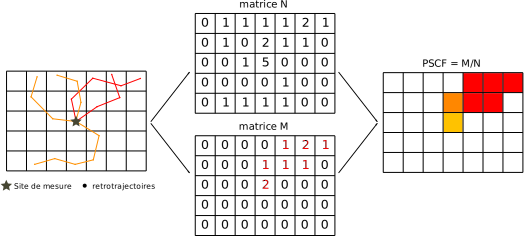
\includegraphics[width=0.9\linewidth]{chapter02/PSCF_method.pdf}
    \caption{Illustration de la méthode PSCF : les rétrotrajectoires depuis le site de
        mesure sont calculées, celles associées à une concentration seuil sont
        représentées en rouge, les autres en orange. Les matrices N et M s'obtiennent par
        simple décompte du nombre de rétrotrajectoires passés dans chaque cellule de
        taille prédéfinies, puis le ratio nous donne une estimation de l'origine
    géographique, représentée ici terme d'intensité de rouge.}%
    \label{fig:chapter02/PSCF_method}
\end{figure}

\subsubsection{Automatisation et simplification : pyPSCF}%
\label{ssub:automatisation_et_simplification_pypscf}

Ces étapes fastidieuses de calcul des rétrotrajectoires et de PSCF ont été automatisés
dans un paquet python, pyPSCF\footnote{Dépot git pyPSCF:
\url{https://gricad-gitlab.univ-grenoble-alpes.fr/webersa/pyPSCF}}, permettant le
traitement d'un grand nombre de rétrotrajectoire en utilisant le modèle lagrangian
HYSPLIT et calculant de manière facilité une PSCF en un site donné, en variant notamment
les différents paramètres succeptibles d'influencer le modèle.

\subsection{Application : Importance et origine géographique du MSA ? (Golly et al. 2019)}%
\label{sub:origine_terrestre_ou_marine_du_msa_}

Comme expliqué précemment, une part importante des aérosols provient de sources
secondaires, c'est-à-dire du vieillissement et des réactions dans l'atmosphère. Une part
importante de ces aérosols secondaires sont d'origines organiques. Les travaux
de~\textcite{gollyOrganic2019}, auxquels j'ai pris part, s'attachent notamment à la
quantification de cette matière organique secondaire, sur 5 sites ruraux en France
pendant l'année 2013, par la mesure de deux espèces issues de processus secondaires : le
MSA et l'oxalate.  Nous avons pu montrer que le MSA, considéré comme provenant de
l'oxydation du DMS, peut contribuer jusqu'à 10 à 20\% de l'OC en période chaude,
indiquant une forte proportion d'aérosols organiques secondaires durant l'été. Mais
surtout, le MSA est considéré comme provenant des émissions de DMS du phytoplanction
marin, au point qu'il est proposé comme méthode de séparation entre le sulfate d'origine
marine et ses autres provenances.

En conduisant une analyses PSCF sur les 25\% des jours les plus fortement chargés en MSA,
nous avons pu confirmer l'importance marine de ce composé, mais également montrer qu'une
part non négligeable semble provenir d'environnement terrigène (voir
figure~\ref{fig:chapter02/golly_PSCF_MSA}), confortant les études suggérants des
processus d'émissions du MSA par des sources biologiques
terrestres~\autocite{bozzettiArgon2017}, pouvant provenir des forêts ou des
sols~\autocite{jardineDimethyl2015,miyazakiSeasonal2012}.

L'une des implications directes de ces travaux résulte en l'ajout systématique du MSA
comme variable d'entrée des études PMF, quelque soit leur localisation. En effet, le
signal du MSA est clairement distinct des autres espèces chimiques mesurées et représente
également une part important de la matière organique. Cette espèce est donc a minima
traceuse de processus secondaires présent sur l'ensemble de l'europe occidental.

\begin{figure}[ht]
    \centering
    \includegraphics[width=0.9\linewidth]{chapter02/golly_PSCF_MSA.png}
    \caption{Probabilité de l'origine géographique du MSA, issue de l'article
        de~\textcite{gollyOrganic2019}. Bien que l'on retrouve l'origine marine du MSA,
        les sites de Dieulefit, OPE ou Peyrusse-Vieille indiquent également une forte
        probabilité d'origine terrestre de ce composé.}%
    \label{fig:chapter02/golly_PSCF_MSA}
\end{figure}

\subsection{Application 2 : Validation des solutions PMF}%
\label{sub:application_2_validation_des_solutions_pmf}

Une autre utilisation de la PSCF consite à croiser les informations issues de la PSCF et
des PMF.
En effet, il n'existe pas de moyen simple de valider le sens géochimique d'une solution
PMF autrement que l'expertise et les connaissances de l'utilisateur.
Une fois une solution obtenu, il est possible de conduire une étude PSCF sur les
différents facteurs identifiés par la PMF. Ainsi, on s'attend à ce que le facteur
\textit{sel de mer} provienne géographiquement d'un océan ou d'une mer. De même la
\textit{combustion de biomasse domestique} ne devrait pas pointer d'emplacement
particulier puisqu'il s'agit d'une source diffuse.

\todo{Exemple de l'OPE : sel de mer et combustion de biomass}


\section{Généralisation d'observations}%
\label{sec:généralisation_dobservations}

\subsection{Mise en place d'une base de donnée harmonisée}%
\label{sub:mise_en_place_d_une_base_de_donnée_harmonisée}

\subsection{Application : Importance des émissions primaires biogéniques (Samaké et al.
2019)}%

\label{sub:application_importance_des_émissions_primaires_biogéniques_samaké_et_al_2019_}


\section{De nouveaux traceurs secondaires pour les PMF ?}%
\label{sec:amélioration_des_solutions_pmf_grâce_à_de_nouveaux_traceurs_organiques}

\subsection{Problématique}%
\label{sub:problématique}

\subsection{Ajout des acides organiques comme traceur du SOA ? (Borlaza et al. in prep)}%
\label{sub:ajout_des_acides_organiques_comme_traceur_du_soa_borlaza_et_al_in_prep_}




\printbibliography[segment=\therefsegment,heading=subbibliography]
